
\section{人体三维姿态估计问题的研究}
\subsection{问题描述}
三维人体姿态估计问题,即是说给定输入的人体图片或视频序列,从中得到人体的三维关节点的位置。从上一节中我们已经得到了人体的二维关节点位置,因此对于这一部分我们需要得到相应的人体三维姿态的估计。但是在只有单个视角的情况下,三维估计具有尺度和深度的不确定性。在只有一个相机的情况下,通常使用各种先验信息来减少这种不确定性,在我们的实验场景下,我们可以利用多个相机的空间信息,来优化求解人体的三维关节点的坐标。

\subsection{模型概述}
\subsubsection{相机模型}
\comment{先写一下相机模型的定义}

\comment{这里写相机标定的内容}
\subsubsection{三角法}
% https://scm_mos.gitlab.io/2018/12/08/triangulate/
对于三维空间中的一点$\bfX$,其在世界坐标系中的表示为
\begin{equation}
    \bfX = [x,y,z,1]^T
\end{equation}
第$i$个相机的参数矩阵为
\begin{equation}
    P_i = K_i[R_i | t_i] = \left[ \begin{array}{c}
        P_{i1} \\ P_{i2} \\ P_{i3}
    \end{array}\right]  
\end{equation}
点$X$在第$i$个相机中的投影的坐标为
\begin{equation}
    \bm{x_i} = (x_i, y_i, 1)^T    
\end{equation}
根据投影方程,即有
\begin{equation}
    \bm{x_i} = P_i\bfX
\end{equation}
上式两边同时叉乘$\bm{x_i}$,即有
\begin{equation}
    \bm{x_i} \times (P_i\bfX) = 0
\end{equation}
展开即可得到:
\begin{align}
    x_i(P_{i3}\bm{X}) &- P_{i1}\bm{X} = 0 \\
    y_i(P_{i3}\bm{X}) &- P_{i2}\bm{X}= 0 \\
    x_i(P_{i2}\bm{X}) &- y_iP_{i1}\bm{X}= 0
\end{align}
第三个方程与前两个方程线性相关,因此该组方程实际只提供了两个自由度,即
\begin{align}
    \left[ \begin{array}{c}
        x_iP_{i3} - P_{i1} \\ y_iP_{i3} - P_{i2}
    \end{array}\right]\bm{X} = \bm{0}
\end{align}
因此每个相机上的一个观察点提供了两个约束,而该点的坐标有三个自由度,因此至少需要两个视角才能解出一个点的坐标。而我们的能用的视角个数大于两个,也就是说需要求解超定方程。即求解超静定的齐次线性方程
\begin{equation}
    AX = \bm{0}
\end{equation}
因此我们采用SVD分解的方法,计算$A$矩阵奇异值最小的对应的奇异向量,就是三维坐标的解。那么我们的问题即为假定未知的所有的关节的三维点的坐标为$S\in \mathbb{R}^{3\times N}$,$N$为关节点的数目,第$i$ 个相机的参数为$R_i,T_i,K_i$。那么该问题的方程可写为:
\begin{equation}
    \left[ \begin{array}{c}
        x_{n0}P_{03} - P_{01} \\ 
        y_{n0}P_{03} - P_{02} \\
        x_{n1}P_{13} - P_{11} \\ 
        y_{n1}P_{13} - P_{12} \\
        \vdots \\
        x_{ni}P_{i3} - P_{i1} \\ 
        y_{ni}P_{i3} - P_{i2} 
    \end{array}\right] \left[ \begin{array}{c}
        X_n \\
        Y_n\\
        Z_n\\
        1 
    \end{array}\right]  = \bm{0}, n = 1,2,\ldots,N
\end{equation}
对于所有关节点,求解方程即可获得所有关节点的三维空间坐标。

\subsubsection{优化法}
由于在实际情况中,我们得到的二维关节点不一定在每个相机下都可见,因此我们需要通过一个权值来控制该关节点在一个相机视角下的可见性。同时,由于深度神经网络的输出带有不确定性,其对每个关节的检测结果均会有一个置信度的指标,置信度大即表示深度神经网络模型认为该点为对应关节的概率大,反之置信度小则表示该点是该关节的不确定性较大。那么我们在恢复人体的三维关节坐标时即可将该权重纳入考虑范围内,即更加相信那些置信度高的视角下的检测结果,通过这种方法来使我们的模型更加鲁棒。

由前文可知,相机投影模型为
\begin{equation}
    Z_i \bm{x_i} = K_i(R_i\bm{X} + T_i)
\end{equation}
投影坐标即为
\begin{equation}
    \bm{x_i} = Z_i^{-1}K_i(R_i\bfX + T_i)    
\end{equation}
那么根据各个视角下的观测到的二维坐标,我们的目标函数可以写为
\begin{equation}
    \min \sum^I_{i=1} \sum_{n=1}^N w_{in}||x_{in} - \hat x_{in}||_2
\end{equation}
将投影坐标表达式代入,即得
\begin{equation}
    \min \sum^I_{i=1} \sum_{n=1}^N w_{in}||Z_i^{-1}K_i(R_iX_n + T_i) - \hat x_{in}||_2  
\end{equation}
\newcommand{\mi}{第\(i\)个}
\newcommand{\mn}{第\(n\)个}
\newcommand{\qczb}{齐次坐标}
其中,$w_{in}$表示\mi 相机视角下,\mn 关节点的对应的深度神经网络检测的二维位置的置信度;$\hat x_{in}$ 表示\mi 相机视角下,\mn 关节点通过深度神经网络估计的在图像平面上的位置;$X_n$为\mn 关节的三维齐次坐标。

\subsection{模型应用}
\comment{写在LightStage数据上采集得到的结果}

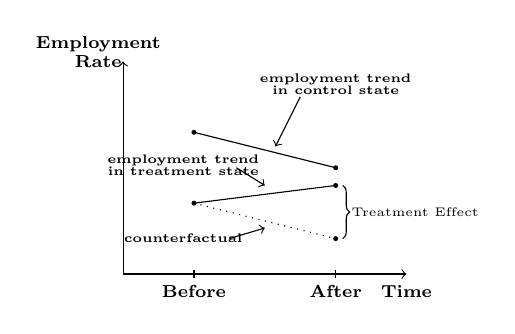
\begin{tikzpicture}[scale=0.9, transform shape]
    %\draw[step=0.5cm,gray,very thin] (0,0) grid (4,3);
    \draw[->] (0,0) -- (4,0) ; 
    \draw[->] (0,0) -- (0,3) ; 
    \draw[-] (1,2) -- (3,1.5); 
    \draw[dotted] (1,1) -- (3,0.5); 
    \draw[-] (1,1) -- (3,1.25);
    \draw[->] (2.5,2.5) -- (2.15,1.8);
    \draw[->] (1.6,1.5) -- (2,1.25); 
    \draw[->] (1.5,0.5) -- (2,0.65); 
    \draw[-] (1,0.05) -- (1,-0.05);
    \draw[-] (3,0.05) -- (3,-0.05);
    \draw[decoration={brace},decorate]
    (3.1,1.25) -- node[right] {{\tiny Treatment Effect}} (3.1,0.5);
    \node at (4,-0.25) {\scriptsize\textbf{Time}};
    \node at (-0.35,3.25) {\scriptsize\textbf{Employment}};
    \node at (-0.35,3) {\scriptsize\textbf{Rate}};
    \node at (1,-0.25) {\scriptsize\textbf{Before}};
    \node at (3,-0.25) {\scriptsize\textbf{After}};
    \node at (3,2.75) {\tiny\textbf{employment trend}};
    \node at (3,2.6) {\tiny\textbf{in control state}};
    \node at (0.85,1.6) {\tiny\textbf{employment trend}};
    \node at (0.85,1.45) {\tiny\textbf{in treatment state}};
    \node at (0.85,0.5) {\tiny\textbf{counterfactual}};
    \fill (1,1) circle[radius=1pt];
    \fill (3,0.5) circle[radius=1pt]; 
    \fill (3,1.5) circle[radius=1pt]; 
    \fill (3,1.25) circle[radius=1pt]; 
    \fill (1,2) circle[radius=1pt]; 
    \end{tikzpicture}